
\begin{figure}[h!]
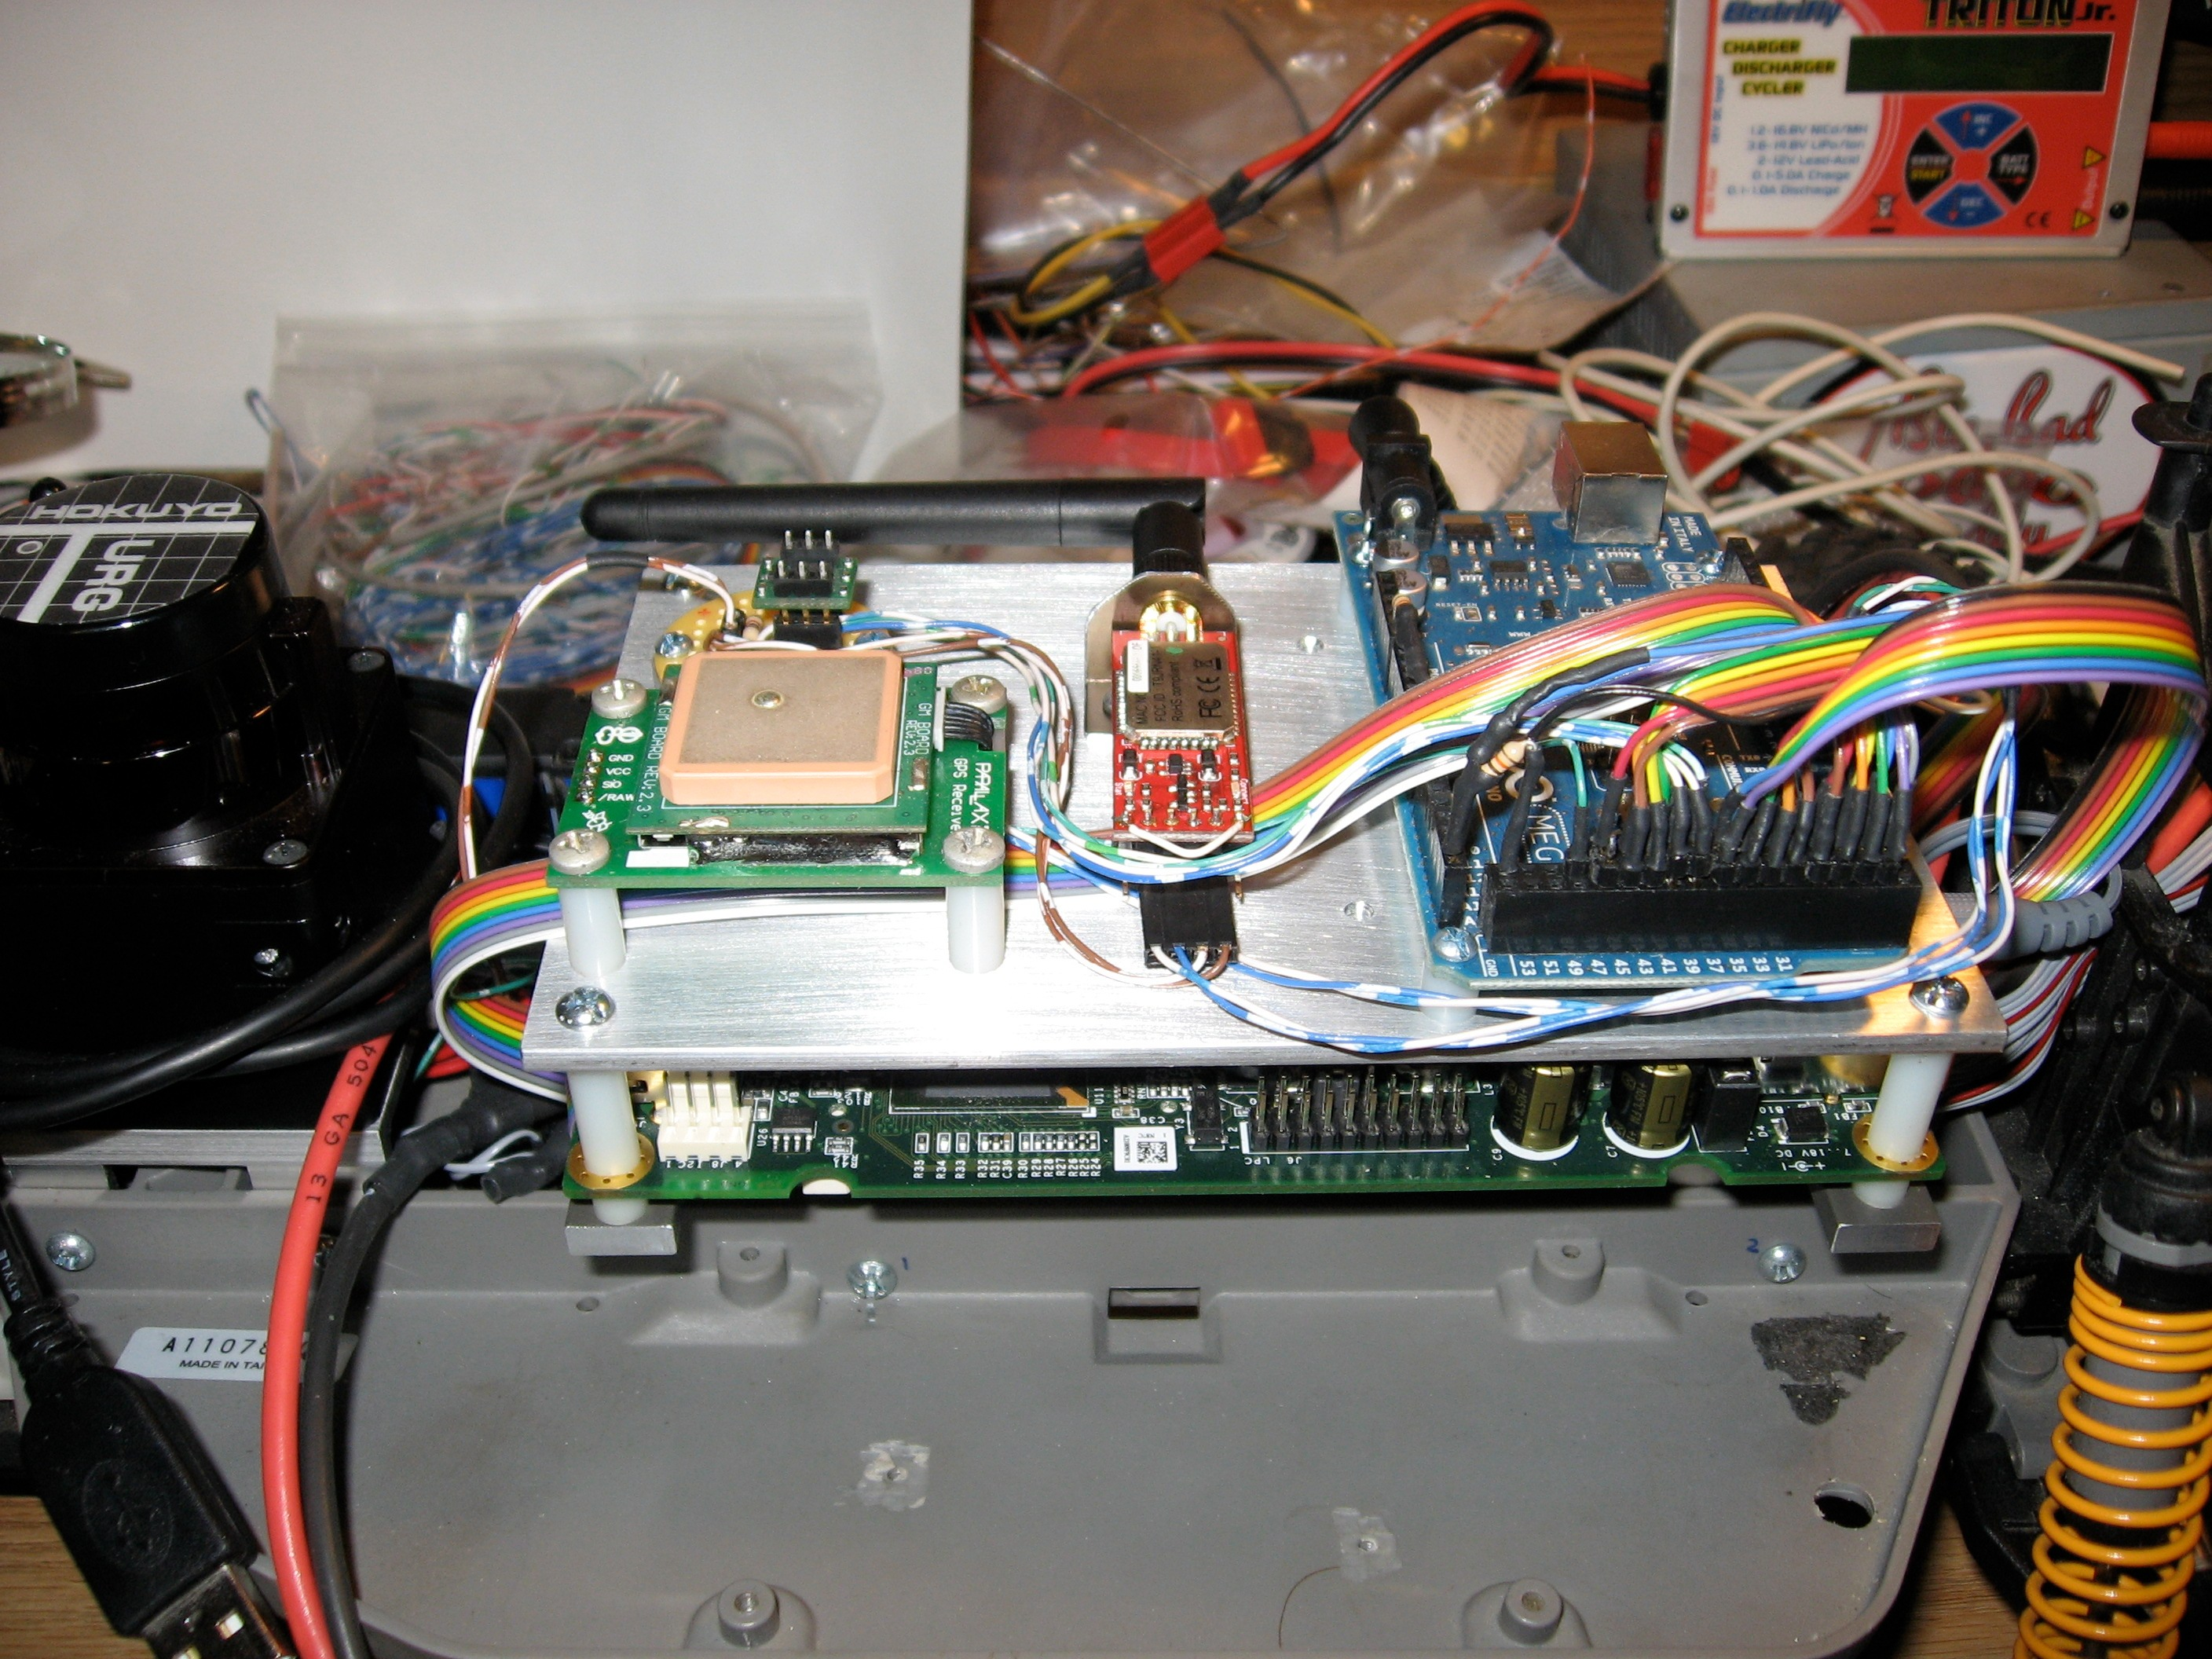
\includegraphics[width=1.0\textwidth]{hardware}
\caption{Internals and sensors}
\end{figure}

I replaced the original wiring and interface circuitry, built from whatever components I had lying around, stuck into a breadboard, with properly selected componenets on a custom perfboard, with color-coded wiring.

I also replaced the original RC motor controller, which had problems switching into reverse, with a motor driver from pololu, driven with PWM generated on the arduino.

The power distribution system consists of two batteries, allowing me to isolate the motor supply from the electronics supply, while sharing a common ground. This provides enough noise isolation that the electronics are unaffected by noise from the motor, which had been a problem in the past.

The sensors are powered by a switching 5V regulator, while the arduino and the primary computer are connected directly to the battery supply voltage. There is also an electonic power cutoff, allowing the electonics to shut off automatically to avoid running the batteries too low. The 5V regulator has an enable line, allowing the sensors to be turned off, should the need arise.
